

\section{Methods}

\subsection{Downloading scripts used in this tutorial}

If one is interested to reproduce the workflow presented here, a good starting point would be to download the following GitHub repository:

\begin{verbatim}
git clone https://github.com/soda460/RNAseq_GATK_JGW.git
\end{verbatim}

It contains all scripts described in this section as well as several text files that allow to easily reproduce the analysis presented here. Note that some scripts use relative paths. Therefore using the files/folder organization presentend in figure 2 will help to reproduce the results presented here with minimal changes.



contained will also make the whole process easier.




\begin{figure}
\begin{center}

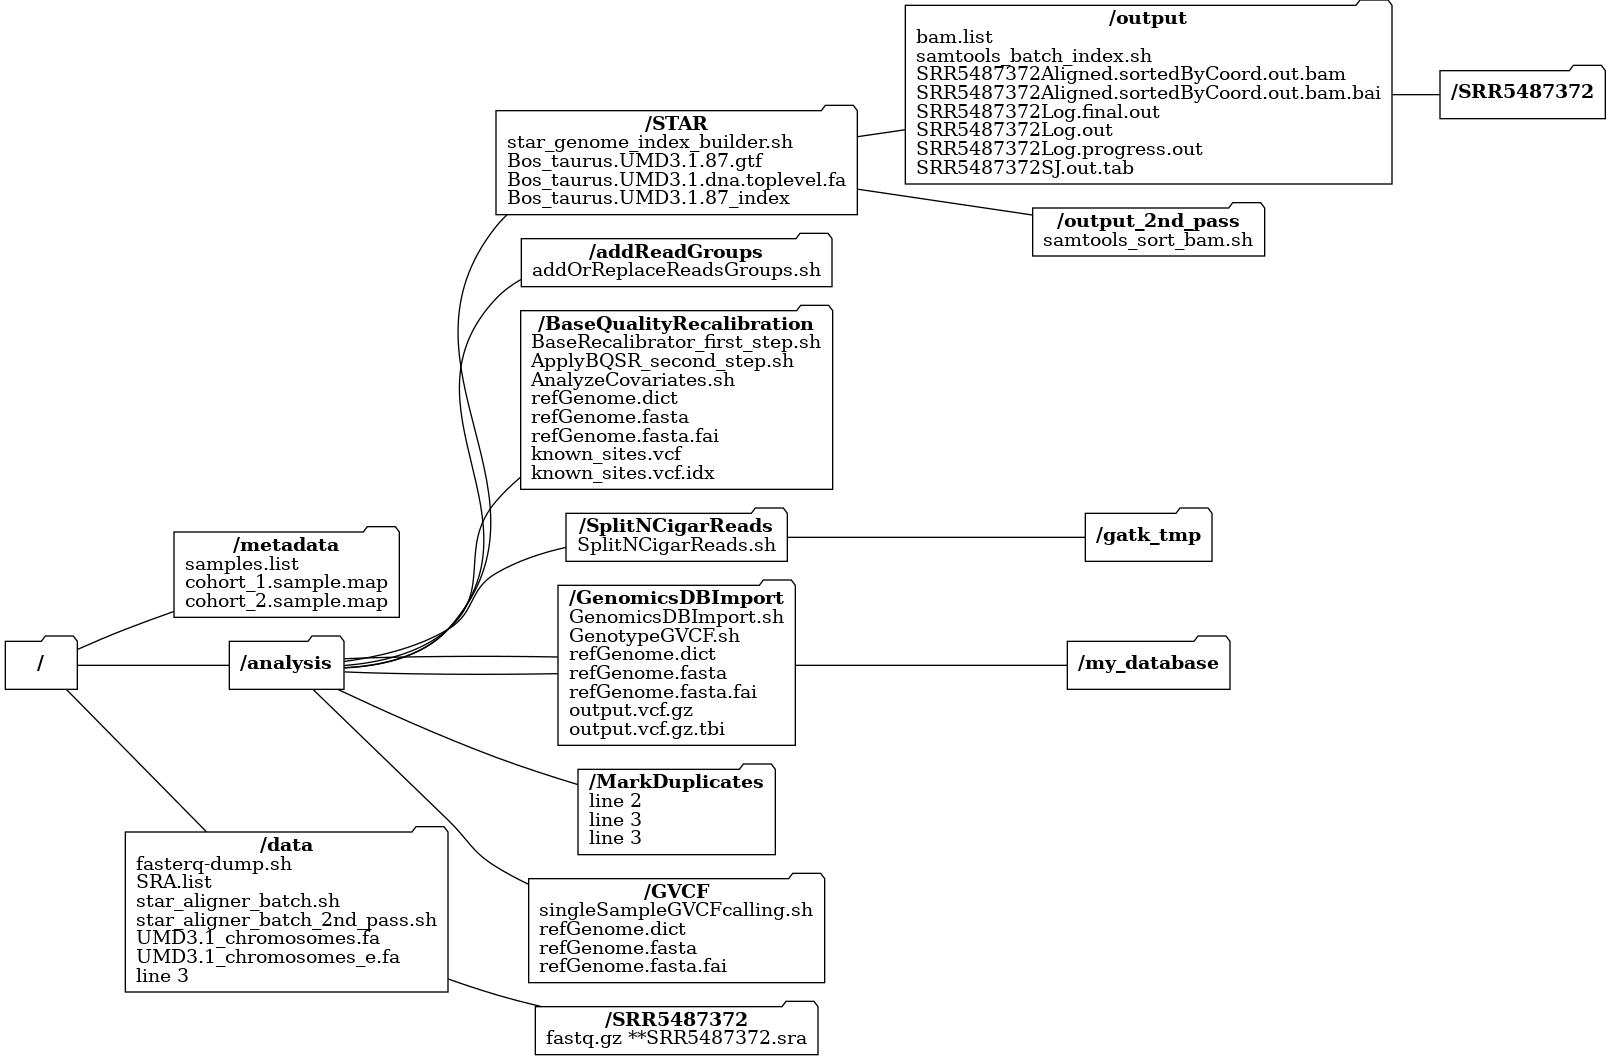
\includegraphics[width=\textwidth]{misc/tree.png}
\caption[caption] {long desc.}

\end{center}
\end{figure}







\subsection{Downloading the MAP dataset from Sequence Read Archive}

We will use the complete RNA-seq raw sequences from \citep{Ariel2021}. However, rather than using the 72 samples presented in the article, we will focus on 24 representative samples of this study:

The \textbf{SRA.list} file contains the SRA identifiers of these 24 samples:
\begin{verbatim}
SRS2153774
SRS2153779
SRS2153781
SRS2153786
SRS2153787
SRS2153791
SRS2153793
SRS2153797
SRS2153799
SRS2153803
SRS2153805
SRS2153809
SRS2153811
SRS2153815
SRS2153817
SRS2153821
SRS2153823
SRS2153827
SRS2153829
SRS2153833
SRS2153835
SRS2153839
SRS2153841
SRS2153845
\end{verbatim}



Navigate to the /data directory and download the 24 samples with the the following command from the SRAtoolkit:

\begin{verbatim}
prefetch --option-file SRA.list
\end{verbatim}

To extract fastq files from .sra files, the fasterq-dump command is required. For example, the following command will produce SRR5487396\_R1.fastq.gz and SRR5487396\_R2.fastq.gz files from the SRR5487396.sra archive.

\begin{verbatim}
fasterq-dump --split-files SRR5487396/SRR5487396.sra
\end{verbatim}

In practice, you will want to extract all downloaded sequence read archives, which are nested in distinct folders. Navigate to the /data folder and use the following qsub command to lauch the faster-qdump commands sequentially:

\begin{verbatim}
qsub faster-qdump.sh
\end{verbatim}

where \textbf{faster-qdump.sh} is a bash script containing instructions for the SGE workload manager and the code to iterate on all downloaded sequence read archives and produce the forward and reverse fastq files:

\begin{verbatim}
#! /bin/bash
#$ -S /bin/bash
#$ -cwd
#$ -N 'fasterq-dump'
#$ -pe smp 12
#$ -o ./qsub_log.txt
#$ -e ./qsub_err.txt
	
for i in `ls -d SRR*`; do
	cd $i
	fasterq-dump --split-files $i.sra
	cd ..
done
\end{verbatim}



However, execute the latter script would take a lot of times. To take advantage of the capacity of the cluster, one should may consider launching array tasks (task in parallel). To learn more about this, one can visit this page (SGE).

Before using the faster-qdump\_parallel.sh, we need to create a simple list file of the 24 SRR* folders present in the /data folder:

\begin{verbatim}
ls -d1 SRR5487???>SRR.list
\end{verbatim}

Be sure that the SRR.list file contains the 24 SRR identifiers (without the .sra extension) on separates lines before lauching the paralle version of fasterq.dump.sh which look like:

\begin{verbatim}
#!/bin/bash
#$ -V
#$ -N fasterq-dump
#$ -S /bin/bash
#$ -cwd
#$ -j y
#$ -b n
#$ -e ./qsub_err.txt
#$ -o ./qsub_log.txt
#$ -q all.q
#$ -t 1-24
#$ -pe smp 4

input=$(head -n $SGE_TASK_ID SRR.list | tail -n 1)

fasterq-dump --split-files $input/$input.sra
\end{verbatim}


Figure x show how a computationnaly intense task, namely the decompressing of an .sra archive, can be run at the same time with different input files. This can be done by using the SGE task array capabilities. Technically, the same script is run multiple times, with different values taken by the single environment variable \$SGE\_TASK\_ID. Since many bioinformatic tasks used in this tutorial are computationally intensive, most of the scripts presented thereafter will be base on this model.




%figure file organization



 

\subsection{Performing STAR alignment}

\subsubsection{Generating genome indexes files}

STAR genomes are available for a limited number of genomes on the gingeras lab. We will use the for \textit{Bos taurus}  UMD3.1.87 annotations file since the BosTau7 version of the genome was used in \cite{Ariel2021}. The GTF file describe all exons whereas the .dna.toplevel.fa fasta file contains the corresponding sequences.



\begin{verbatim}
wget http://labshare.cshl.edu/shares/gingeraslab/www-data/dobin/\
STAR/STARgenomes/Old/ENSEMBL/bos_taurus/Bos_taurus.UMD3.1.87.gtf;

wget http://labshare.cshl.edu/shares/gingeraslab/www-data/dobin/\
STAR/STARgenomes/Old/ENSEMBL/bos_taurus/Bos_taurus.UMD3.1.dna.toplevel.fa;
\end{verbatim}

To prepare genome index files for STAR, use the genomeGenerate built-in STAR command.
Note that you have to create a directory where STAR could buid the index.

\begin{verbatim}
mkdir Bos_taurus.UMD3.1.87_index
\end{verbatim}

 as in the following script:

\begin{verbatim}
cat Bos_taurus.UMD3.1.87_index/chrName.txt | head -n 34
\end{verbatim}

\textbf{star\_genome\_index\_builder.sh}
\begin{verbatim}
#! /bin/bash
#$ -S /bin/bash
#$ -cwd
#$ -N 'STAR_genome_builder'
#$ -pe smp 6
#$ -o ./qsub_log.txt
#$ -e ./qsub_err.txt
STAR --runThreadN 6 \
--runMode genomeGenerate \
--genomeDir Bos_taurus.UMD3.1.87_index \
--genomeFastaFiles ./Bos_taurus.UMD3.1.dna.toplevel.fa \
--sjdbGTFfile ./Bos_taurus.UMD3.1.87.gtf \
--sjdbOverhang 99
\end{verbatim}






\subsubsection{Aligment with the STAR aligner}

At this step, we align our raw .fastq files with the STAR aligner.

%STAR fisrt pass
\begin{verbatim}
#!/bin/bash
#$ -V
#$ -N 'STAR_aligner'
#$ -S /bin/bash
#$ -cwd
#$ -j y
#$ -b n
#$ -e e
#$ -o STAR_aligner_1st_pass.$TASK_ID.log
#$ -q all.q
#$ -t 1-24
#$ -pe smp 4


input=$(head -n $SGE_TASK_ID SRR.list | tail -n 1)


mkdir -p ../analysis/STAR/output/$input

STAR --genomeDir ./Bos_taurus.UMD3.1.87_index \
--runThreadN 12 \
--readFilesIn  ./$input/$input"_1.fastq" ./$input/$input"_2.fastq" \
--outFileNamePrefix ../analysis/STAR/output/$input \
--outSAMtype BAM SortedByCoordinate \
--outSAMunmapped Within \
--outSAMattributes Standard
\end{verbatim}



\subsubsection{Adding Splice junctions (2nd mapping pass)}

GATK workflow recommend to perform 2-pass mapping with the STAR aligner. The 2nd mapping pass is identical to the first alignment except that all splice junctions discovered in the first pass are given as input to the programs, allowing to XXXX. Simply specify a list of all splice junctions files after the --sjdbFileChrStartEnd argument.


\begin{verbatim}
----outTmpDir ../analysis/STAR/output_2nd_pass/_STARtmp_$TASK_ID \
\end{verbatim}

%STAR 2nd pass listing
\begin{verbatim}
#!/bin/bash
#$ -V
#$ -N 'STAR_aligner_2nd_pass'
#$ -S /bin/bash
#$ -cwd
#$ -j y
#$ -b n
#$ -e e
#$ -o STAR_aligner_2nd_pass.$TASK_ID.log
#$ -q all.q
#$ -t 1-24
#$ -pe smp 4


input=$(head -n $SGE_TASK_ID SRR.list | tail -n 1)

mkdir -p ../analysis/STAR/output_2nd_pass/$input

STAR --genomeDir ./Bos_taurus.UMD3.1.87_index \
--runThreadN 4 \
--readFilesIn  ./$input/$input"_1.fastq" ./$input/$input"_2.fastq" \
--outFileNamePrefix ../analysis/STAR/output_2nd_pass/$input \
--outSAMtype BAM SortedByCoordinate \
--outSAMunmapped Within \
--outSAMattributes Standard \
--outTmpDir ../analysis/STAR/output_2nd_pass/_STARtmp_$SGE_TASK_ID \
--sjdbFileChrStartEnd \
../analysis/STAR/output/SRR5487372SJ.out.tab \
../analysis/STAR/output/SRR5487384SJ.out.tab \
../analysis/STAR/output/SRR5487396SJ.out.tab \
../analysis/STAR/output/SRR5487408SJ.out.tab \
../analysis/STAR/output/SRR5487420SJ.out.tab \
../analysis/STAR/output/SRR5487432SJ.out.tab \
../analysis/STAR/output/SRR5487376SJ.out.tab \
../analysis/STAR/output/SRR5487388SJ.out.tab \
../analysis/STAR/output/SRR5487400SJ.out.tab \
../analysis/STAR/output/SRR5487412SJ.out.tab \
../analysis/STAR/output/SRR5487424SJ.out.tab \
../analysis/STAR/output/SRR5487436SJ.out.tab \
../analysis/STAR/output/SRR5487378SJ.out.tab \
../analysis/STAR/output/SRR5487390SJ.out.tab \
../analysis/STAR/output/SRR5487402SJ.out.tab \
../analysis/STAR/output/SRR5487414SJ.out.tab \
../analysis/STAR/output/SRR5487426SJ.out.tab \
../analysis/STAR/output/SRR5487438SJ.out.tab \
../analysis/STAR/output/SRR5487382SJ.out.tab \
../analysis/STAR/output/SRR5487394SJ.out.tab \
../analysis/STAR/output/SRR5487406SJ.out.tab \
../analysis/STAR/output/SRR5487418SJ.out.tab \
../analysis/STAR/output/SRR5487430SJ.out.tab \
../analysis/STAR/output/SRR5487442SJ.out.tab

\end{verbatim}



\subsubsection{Sorting alignment files}


After you align your sequences. You will want that your .bam files to be indexed and sorted by coordinates. As mentioned earlier, STAR allows the output to be sorted by coordinates. If you have carefully followed this tutorial, there is no need to sort again your bam files and you can safely ignore the next step and jump to the next subheading. However, if for any reasons, your aligmnents files are not sorted adequately, the sort option of samtools is as easy as :

\begin{verbatim}
samtools sort file.bam -o file_sorted.bam
\end{verbatim}

In a folder containing unsorted alignment, first prepare a list of bam files to be sorted with:

\begin{verbatim}
ls -1 *.bam > bam.list
\end{verbatim}

For our data, a qsub script would allow to re-sort our alignments files:


% samtools sort listing
\begin{verbatim}
#!/bin/bash
#$ -V
#$ -N samtools_sort
#$ -S /bin/bash
#$ -cwd
#$ -j y
#$ -b n
#$ -e e
#$ -o o
#$ -q all.q
#$ -t 1-24
#$ -pe smp 2

input=$(head -n $SGE_TASK_ID bam.list | tail -n 1 | xargs basename -s '.bam')

samtools sort $input.bam -o $input"_sorted.bam"

\end{verbatim}

Note that this listing could be used as a template to perform a variety of samtools subcommands that involve renaming the output files.


\subsubsection{Indexing alignment files}

BAM files (the binary analog of Sequence Alignment Mapping (SAM) files) are very efficient bioinformatic files designed to store high-throughput alignment data. Typically, they contains the result of the alignment of millions of sequencing reads against a reference genome and greatly from being accompagnied with index files for faster random access to the aligned reads. In practice most programs will simply don't work without  

 
BAM files need to be sorted before being indexed

To index all bam files present in the STAR output_2nd_pass folder, first prepare a list of bam files to be indexed with:

\begin{verbatim}
ls -1 *.bam > bam.list
\end{verbatim}

then, you can index all alignements in parallel with:

\begin{verbatim}
qsub samtools_batch_index.sh
\end{verbatim}

where the latter script looks like:

%samtools index listing
\begin{verbatim}
#!/bin/bash
#$ -V
#$ -N samtools_index
#$ -S /bin/bash
#$ -cwd
#$ -j y
#$ -b n
#$ -e e
#$ -o o
#$ -q all.q
#$ -t 1-24
#$ -pe smp 2

input=$(head -n $SGE_TASK_ID bam.list | tail -n 1)

samtools index $input
\end{verbatim}





\subsection{Adding Read groups}

Contrarily to fastq, SAM files have the capacity to handle large amount of metadata. A good practice would be to include informations about the reference genome and the samples in aligment files. Informations about the processing steps could also figure in alignment files. Many programs will add this metadata information when manipulating SAM files.


Before running any GATK workflow, one will need to add Read groups. This step ensure that relevant informations about the sequencing process are assigned to each read in an alignment file. When this step is done carefully, it allow to correct sequencing biais that could arise from...


Here, we will set the flowcells, sequencing lanes and sample barcode in the platform unit (PU) tag.

Before running the main script, we will extract some important columns from our metadata file and place them in separate files that will be used to populate important fields of the read groups. Given metadata from our 24 samples:

\begin{verbatim}
sample,cowID,SRAID,Run,RGPU
A_CTL24,cowA,SRS2153774,SRR5487372,C5NL3ACXX.1.CAGATC
A_MAP24,cowA,SRS2153779,SRR5487376,C5NL3ACXX.1.TGACCA
B_CTL24,cowB,SRS2153781,SRR5487378,C5NL3ACXX.3.TGACCA
B_MAP24,cowB,SRS2153786,SRR5487382,C5NL3ACXX.3.GTGAAA
C_CTL24,cowC,SRS2153787,SRR5487384,C5K8FACXX.3.AGTCAA
C_MAP24,cowC,SRS2153791,SRR5487388,C5K8FACXX.3.GTCCGC
D_CTL24,cowD,SRS2153793,SRR5487390,C5K8FACXX.1.TGACCA
D_MAP24,cowD,SRS2153797,SRR5487394,C5K8FACXX.1.GTGAAA
E_CTL24,cowE,SRS2153799,SRR5487396,C547FACXX.1.AGTCAA
E_MAP24,cowE,SRS2153803,SRR5487400,C547FACXX.1.GTCCGC
F_CTL24,cowF,SRS2153805,SRR5487402,C547FACXX.3.TGACCA
F_MAP24,cowF,SRS2153809,SRR5487406,C547FACXX.3.GTGAAA
G_CTL24,cowG,SRS2153811,SRR5487408,C5NL3ACXX.5.AGTCAA
G_MAP24,cowG,SRS2153815,SRR5487412,C5NL3ACXX.5.GTCCGC
H_CTL24,cowH,SRS2153817,SRR5487414,C5NL3ACXX.7.TGACCA
H_MAP24,cowH,SRS2153821,SRR5487418,C5NL3ACXX.7.CTTGTA
I_CTL24,cowI,SRS2153823,SRR5487420,C5K8FACXX.5.AGTTCC
I_MAP24,cowI,SRS2153827,SRR5487424,C5K8FACXX.5.GTGAAA
J_CTL24,cowJ,SRS2153829,SRR5487426,C5K8FACXX.7.TGACCA
J_MAP24,cowJ,SRS2153833,SRR5487430,C5K8FACXX.7.GTGAAA
K_CTL24,cowK,SRS2153835,SRR5487432,C547FACXX.5.AGTCAA
K_MAP24,cowK,SRS2153839,SRR5487436,C547FACXX.5.GTCCGC
L_CTL24,cowL,SRS2153841,SRR5487438,C547FACXX.7.AGTCAA
L_MAP24,cowL,SRS2153845,SRR5487442,C547FACXX.7.GTCCGC
\end{verbatim}

The following commands will produce 
The RGLB.txt file will hold the library name. In this case, we will use the sample name.
The RGPU is more complex. IT contains informations about X, Y and Z.



\begin{verbatim}
# Corresponding to the sample name
cut -f 1 -d ',' ../../metadata/metadata.txt | tail -n +2 > RGLB.txt
 
# Corresponding to the PU tag FLOW CELL 
cut -f 5 -d ',' ../../metadata/metadata.txt | tail -n +2 > RGPU.txt
\end{verbatim}





%AddOrReplaceReadGroups listing
\begin{verbatim}
#!/bin/bash
#$ -V
#$ -N AddOrReplaceReadGroups
#$ -S /bin/bash
#$ -cwd
#$ -j y
#$ -b n
#$ -e e
#$ -o logfile.txt
#$ -q all.q
#$ -t 1-24
#$ -pe smp 1

eval "$(conda shell.bash hook)"
conda activate gatk4	

SAMPLES="$HOME/jsb/springer/metadata/samples.list"
BAMPATH="$HOME/jsb/springer/analysis/STAR/output_2nd_pass"
OUTPUT="$HOME/jsb/springer/analysis/addReadGroups"	

readarray -t RGLB < ./RGLB.txt
readarray -t RGPU < ./RGPU.txt

input=$(head -n $SGE_TASK_ID $SAMPLES | tail -n 1)	

java -jar $PICARD AddOrReplaceReadGroups \
	I=$BAMPATH/$input"Aligned.sortedByCoord.out.bam" \
	O=$OUTPUT/$input".bam" \
	RGLB=$RGLB \
	RGPL=ILLUMINA \
	RGPU=$RGPU \
	RGSM=$input
	
conda deactivate
\end{verbatim}


To validate that the reads groups have been correctly, you could use this simple trick on the .bam files:

\begin{verbatim}
samtools view -H sample.bam | grep '@RG' 
\end{verbatim}






\subsection{MarkDuplicates}








Duplicate reads can arise from PCR duplication artifacts that take place during the library construction or from reading errors that occur during the sequencing process (optical duplicates). Regardless of their origin, these reads need to be identified in alignment files. The MarkDuplicate program from the picard tools have many options to deal with these issue and output some metrics. For example, the program offer the possibility to completey remove the duplicate reads and to make the distinction between optical and PCR duplicates.

Since this tool require a



Here we simply identified the duplicate reads:

%MarkDuplicate script
\begin{verbatim}
#!/bin/bash
#$ -V
#$ -N samtools_index
#$ -S /bin/bash
#$ -cwd
#$ -j y
#$ -b n
#$ -o logfile.$TASK_ID.log
#$ -q all.q
#$ -t 1-24
#$ -pe smp 2

SAMPLES="$HOME/jsb/springer/metadata/samples.list"
BAMPATH="$HOME/jsb/springer/analysis/addReadGroups"
OUTPUT="$HOME/jsb/springer/analysis/MarkDuplicates"

input=$(head -n $SGE_TASK_ID $SAMPLES | tail -n 1)

java -jar $PICARD MarkDuplicates \
I=$BAMPATH/$input".bam" \
O=$OUTPUT/$input"_marked_duplicates.bam" \
M=$OUTPUT/$input"_marked_dup_metrics.txt"
\end{verbatim}





BaseRecalibration
IndexFeatureFile

gatk IndexFeatureFile -input jsb.vcf


\subsubsection{The gff3 file}

With the command below, one can see the number of features annotated for each ID in the gff3 file: 

\begin{verbatim}{bash}
cat Ensembl79_UMD3.1_genes.gff3 | cut -f 1 | uniq -cd
\end{verbatim}


%output of cat Ensembl79 gff3
The result of this command is:
\begin{verbatim}
21287 GK000001.2
18819 GK000030.2
26235 GK000002.2
29793 GK000003.2
29598 GK000005.2
18201 GK000004.2
15375 GK000006.2
16534 GK000008.2
28038 GK000007.2
24860 GK000011.2
12861 GK000009.2
23581 GK000010.2
9839 GK000012.2
17254 GK000015.2
11207 GK000014.2
18771 GK000013.2
17134 GK000016.2
14916 GK000017.2
8554 GK000020.2
13262 GK000021.2
26279 GK000018.2
30597 GK000019.2
7463 GK000024.2
15631 GK000022.2
14696 GK000023.2
10159 GK000026.2
14729 GK000029.2
8317 GK000028.2
5227 GK000027.2
17365 GK000025.2
14 GJ058430.1
31 GJ058425.1
3 GJ059486.1
4 GJ058433.1
16 GJ058437.1
15 GJ058424.1
12 GJ060129.1
12 GJ059670.1
124 AY526085.1
24 GJ059556.1
9 GJ059463.1
13 GJ060118.1
19 GJ060120.1
16 GJ060032.1
23 GJ059509.1
3 GJ058729.1
3 GJ060027.1
3 GJ058256.1
\end{verbatim}

Therefore, to ensure that the gff3 chromosome IDs match those presennt in our alignment files, we need to slightly edit this file to replace the pattern used for the chromosome IDs (GK + 0000 + chromosome number) by solely the chromosome number. This could be done easily with sed:

\begin{verbatim}
sed -r s'/^GK[0]+([0-9]+).2/\1/'g Ensembl79_UMD3.1_genes.gff3 > Ensembl79_UMD3.1_genes_e.gff3
\end{verbatim}

Obvisouly it is good idea to inspect the edited file to ensure that the desired changes have been done properly.

\subsection{SplitNCigarReads}

The next step is very specific to RNAseq. Briefly, during this step reads that match align over distinct exons are split and blah.

However, before doing this step, we need to get and prepare reference genome files.

\subsubsection{Prepare reference genome files}

Until now, we have work with STAR reference genome which barely contains sequences that are transcribed in RNA. In order to produce alignments files that will adequately represent reads that span splice junctions, the SplitNCigarReads command require the complete reference sequence. At this point, pay attention to download the same version of the refence genome as the one that was used to prepare the STAR genome.

To get the UMD3.1 assembly, visit \href{https://bovinegenome.elsiklab.missouri.edu/}{https://bovinegenome.elsiklab.missouri.edu/} and download the UMD3.1\_chromosomes.fa.gz and Ensembl79\_UMD3.1\_genes.gff3.gz files. If you inspect the headers of the UMD3.1\_chromosomes.fa, you will notice that each fasta entry contains many fields (e.g. gnl , UMD3.1 Accession numbers). To inspect the fasta headers, simply use grep:

\begin{verbatim}
grep ">" UMD3.1_chromosomes.fa
\end{verbatim}


\begin{verbatim}
>gnl|UMD3.1|GK000010.2 Chromosome 10 AC_000167.1
>gnl|UMD3.1|GK000011.2 Chromosome 11 AC_000168.1
>gnl|UMD3.1|GK000012.2 Chromosome 12 AC_000169.1
...
>gnl|UMD3.1|GJ060407.1 GPS_000344847.1 NW_003101152.1
>gnl|UMD3.1|GJ060408.1 GPS_000344848.1 NW_003101153.1
\end{verbatim}


It is crucial that entries in the reference genome match the corresponding ones in the STAR genome. One could use the following commands to rename the complicated chromosome entries from the UMD3.1 genome to the plain chromosome numbers as what is seen in the STAR genome:

\begin{verbatim}
sed -r s'/^>.+Chromosome\s+(\S+)\s+.+/>\1/' UMD3.1_chromosomes.fa > temp1.fa
grep ">" temp1.fa | head -n 40
sed -r s'/^>gnl\|UMD3\.1\|(\S+)+\s+.+/>\1/' temp1.fa > temp2.fa
grep ">" temp2.fa | tail -n +30 | head -n 10
mv temp2.fa refGenome.fasta
rm temp1.fa
\end{verbatim}


Along with the reference genome, many GATK tools will need a dictionary file ending in .dict and an index file ending in .fai.\href{ https://gatk.broadinstitute.org/hc/en-us/articles/360035531652-FASTA-Reference-genome-format} { https://gatk.broadinstitute.org/hc/en-us/articles/360035531652-FASTA-Reference-genome-format}). These files need to share the same basename as the reference genome. You can prepare the index with:

\begin{verbatim}
samtools faidx refGenome.fasta
\end{verbatim}

Use the GATK CreateSequenceDictionary tool to create the required .dict file:

\begin{verbatim}
gatk CreateSequenceDictionary -R refGenome.fasta
\end{verbatim}

\subsubsection{Run SplitNCigarReads}

Here the listing for the SplitNCigarReads step:

%SplitNCigarReads listing
\begin{verbatim}
#!/bin/bash
#$ -V
#$ -N SplitNCigarReads
#$ -S /bin/bash
#$ -cwd
#$ -j y
#$ -b n
#$ -e e
#$ -o SplitNCigarReads.$TASK_ID.log
#$ -q all.q
#$ -t 1-24
#$ -pe smp 4

eval "$(conda shell.bash hook)"
conda activate gatk4

SAMPLES="$HOME/jsb/springer/metadata/samples.list"
BAMPATH="$HOME/jsb/springer/analysis/MarkDuplicates"
OUTPUT="$HOME/jsb/springer/analysis/SplitNCigarReads"

input=$(head -n $SGE_TASK_ID $SAMPLES | tail -n 1)

gatk SplitNCigarReads \
-R refGenome.fasta \
-I $BAMPATH/$input"_marked_duplicates.bam" \
-O $OUTPUT/$input"_SplitNCigarReads.bam" \
--tmp-dir $output/gatk_tmp

conda deactivate
\end{verbatim}




\subsection{Base Quality Recalibration}

This optional step is highly recommended by 


\subsubsection{BaseRecalibrator first step}
%BaseRecalibrator first script
\begin{verbatim}
#!/bin/bash
#$ -V
#$ -N BaseRecalibrator
#$ -S /bin/bash
#$ -cwd
#$ -j y
#$ -b n
#$ -e e
#$ -o BaseQualityRecalibration_$TASK_ID.log
#$ -q all.q
#$ -t 1-24
#$ -pe smp 4

eval "$(conda shell.bash hook)"
conda activate gatk4

SAMPLES="$HOME/jsb/springer/metadata/samples.list"
BAMPATH="$HOME/jsb/springer/analysis/SplitNCigarReads"
OUTPUT="$HOME/jsb/springer/analysis/BaseQualityRecalibration"

input=$(head -n $SGE_TASK_ID $SAMPLES | tail -n 1)

gatk BaseRecalibrator \
-R ./refGenome.fasta \
-I $BAMPATH/$input"_SplitNCigarReads.bam" \
--known-sites ./jsb.vcf \
-O $OUTPUT/$input"_recal_data.table"

conda deactivate
\end{verbatim}


In the second step of the BaseQuality recalibration, GATK use the content in the .table files to recalibrate base quality.


\subsubsection{BaseRecalibrator second step}
%ApplyBQSR listing
\begin{verbatim}
#!/bin/bash

#$ -V
#$ -N ApplyBQSR
#$ -S /bin/bash
#$ -cwd
#$ -j y
#$ -b n
#$ -e e
#$ -o ApplyBQSR_$TASK_ID.log
#$ -q all.q
#$ -t 1-24
#$ -pe smp 4

eval "$(conda shell.bash hook)"
conda activate gatk4

SAMPLES="$HOME/jsb/springer/metadata/samples.list"
BAMPATH="$HOME/jsb/springer/analysis/SplitNCigarReads"
OUTPUT="$HOME/jsb/springer/analysis/BaseQualityRecalibration"


echo $SAMPLES
input=$(head -n $SGE_TASK_ID $SAMPLES | tail -n 1)

gatk ApplyBQSR \
-R ./refGenome.fasta \
-I $BAMPATH/$input"_SplitNCigarReads.bam" \
--bqsr-recal-file $OUTPUT/$input"_recal_data.table" \
-O $OUTPUT/$input"_recal.bam"

conda deactivate
\end{verbatim}






\subsection{Variant Calling}

More details about the incremental discovery can be found here:

\subsubsection{GVCF part}
%GCVF listing
\begin{verbatim}
#!/bin/bash
#$ -V
#$ -N callingGVCF
#$ -S /bin/bash
#$ -cwd
#$ -j y
#$ -b n
#$ -e e
#$ -o singleSampleCallingGVCF_$TASK_ID.log
#$ -q all.q
#$ -t 1-24
#$ -pe smp 4

eval "$(conda shell.bash hook)"
conda activate gatk4

SAMPLES="$HOME/jsb/springer/metadata/samples.list"
BAMPATH="$HOME/jsb/springer/analysis/BaseQualityRecalibration"
OUTPUT="$HOME/jsb/springer/analysis/GVCF"

echo $SAMPLES
input=$(head -n $SGE_TASK_ID $SAMPLES | tail -n 1)

gatk --java-options "-Xmx4g" HaplotypeCaller \
-R ./refGenome.fasta \
-I $BAMPATH/$input"_recal.bam" \
-O $OUTPUT/$input".g.vcf.gz" \
-ERC GVCF

conda deactivate
\end{verbatim}





\subsubsection{Import DBI }

DBI import

%GenomicsDBImport listing
\begin{verbatim}
eval "$(conda shell.bash hook)"
conda activate gatk4

SAMPLES="$HOME/jsb/springer/metadata"
OUTPUT="$HOME/jsb/springer/analysis/GenomicsDBImport"

gatk --java-options "-Xmx4g -Xms4g" \
GenomicsDBImport \
--genomicsdb-workspace-path $OUTPUT/"my_database" \
-L 1 \
-L 2 \
-L 3 \
-L 4 \
-L 5 \
-L 6 \
-L 7 \
-L 8 \
-L 9 \
-L 10 \
-L 11 \
-L 12 \
-L 13 \
-L 14 \
-L 15 \
-L 16 \
-L 17 \
-L 18 \
-L 19 \
-L 20 \
-L 21 \
-L 22 \
-L 23 \
-L 24 \
-L 25 \
-L 26 \
-L 27 \
-L 28 \
-L 29 \
--sample-name-map $SAMPLES/"cohort_1.sample_map" \
--tmp-dir $HOME/jsb/tmp \
--reader-threads 5
conda deactivate

\end{verbatim}










\subsubsection{Genotype GVCF}

The final step in variant calling can be done with GATK GenotypeGVCFs program.

%GenotypeGVCFs listing
\begin{verbatim}
#!/bin/bash
#$ -V
#$ -N GenotypeGVCF
#$ -S /bin/bash
#$ -cwd
#$ -j y
#$ -b n
#$ -e e
#$ -o GenotypeGVCF.log
#$ -q all.q
#$ -pe smp 4

eval "$(conda shell.bash hook)"
conda activate gatk4

gatk --java-options "-Xmx4g" GenotypeGVCFs \
-R refGenome.fasta \
-V gendb://my_database \
-O output.vcf.gz
conda deactivate
\end{verbatim}






\subsection{Examine and visualize alignment files}

At this step, you could examine your alignments files.

Tablet (https://ics.hutton.ac.uk/tablet/download-tablet/) is a good program to visualize alignments files. The IVG viewer could also be used.


You should keep a copy of the vcf output file in a safe place. It is fairly common to corrput a .gz file with compressing/decompressing operations.





gunzip -c output.vcf.gz > output.vcf
